\subsection{Pre-processing}\label{subsec:chp3img-reg:prepro}
Three different groups of pre-processing methods are commonly applied to images
as initial stage in \acp{cad} for \ac{cap}.
These methods are explained for both \ac{mri} and \ac{mrsi} modalities

\subsubsection{\acs*{mri} modalities}\label{subsubsec:ch3:mriprepro}

\setenumerate{listparindent=\parindent,itemsep=10px}
\setlist{noitemsep}
\begin{enumerate}[leftmargin=*]

\begin{figure}
  \centering
  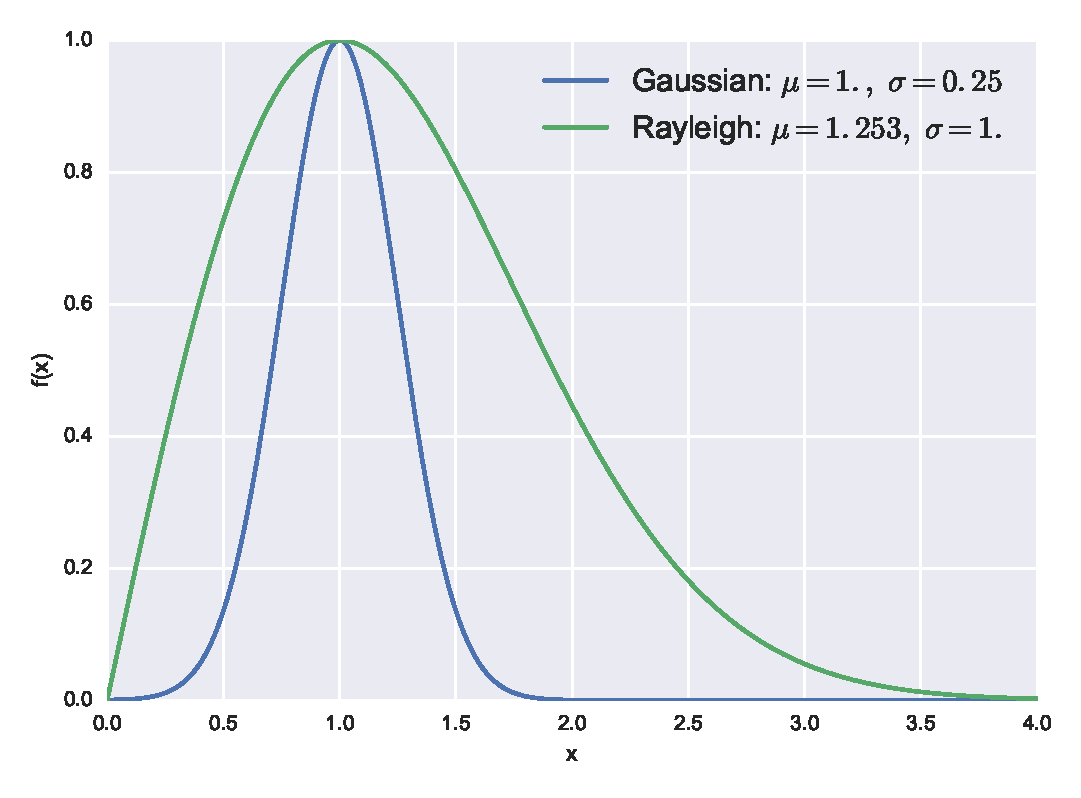
\includegraphics[width=0.7\linewidth]{3_review/figures/processing/pre-processing/noise/noisedistr.eps}
  \caption[Illustration of a Gaussian and Rayleigh distributions.]{Illustration
    of a Gaussian and Rayleigh distribution. Although the mode of these
    distributions are identical, it can be noted that the Rayleigh distribution
    ($\mu=1.253$) is suffering of a bias term when compared with the Gaussian
    distribution ($\mu=1$).}
  \label{fig:noisedistr}
\end{figure}

% Noise filtering
\item[] \textbf{Noise filtering}
The \ac{nmr} signal, measured and acquired in the k-space, is affected by noise.
This noise obeys a complex Gaussian white noise mainly due to thermal noises in
the patient~\cite{Nowak1999}.
Furthermore, \ac{mri} images visualized by radiologists are in fact the
magnitude images resulting from the complex Fourier transform of the k-space
data.
The complex Fourier transform does not affect the Gaussian noise
characteristics since this is a linear and orthogonal
transform~\cite{Nowak1999}.
However, the calculation of the magnitude is a non-linear transform --- i.e.,
the square root of the sum of squares of real and the imaginary parts ---
implying that the noise distribution is no longer Gaussian; it indeed follows a
Rician distribution making the denoising task more challenging.
Briefly, a Rician distribution is characterized as follows: in low-\ac{si}
region (low-\ac{snr}), it can be approximated with a Rayleigh distribution
while in high-\ac{si} region (high-\ac{snr}), it is similar to a Gaussian
distribution~\cite{Manjon2008}.
Refer to \acs{fig}\,\ref{fig:noisedistr} to observe the difference between a
Gaussian and a Rayleigh distribution.
Comprehensive reviews regarding denoising methods can be found
in~\cite{Buades2005,Mohan2014}.

Median filtering is the simplest approach used to address the denoising issue
in \ac{mri} images~\cite{Ozer2009,Ozer2010}.
In both studies, \citeauthor{Ozer2010}~\cite{Ozer2009,Ozer2010} used a
square-shaped kernel of size \SI[product-units=repeat]{5x5}{\px}.

More recently, \citeauthor{rampun2016quantitative} used a combination of median
and anisotropic diffusion
filter~\cite{rampun2015classifying,rampun2016computer,rampun2016computerb,rampun2016quantitative},
proposed in~\cite{ling2002smoothing}.
In low-\ac{snr} images, the gradient generated by an edge and noise can be
similar, making the denoising by diffusion more challenging.
In this condition, the threshold allowing to locally differentiate a noise
gradient from an edge gradient needs to be increased, at the cost of blurring
edges after filtering.
Therefore, \citeauthor{ling2002smoothing}~\cite{ling2002smoothing} proposed to
apply a standard anisotropic diffusion filter with a low threshold followed by
a median filtering to remove large noise spikes.



\citeauthor{samarasinghe2016semi} filtered \ac{dce}-\ac{mri} images with a
sliding 3D Gaussian filter~\cite{samarasinghe2016semi}.
However, from a theoretical point of view, this simple filtering method is not
well formalized to address the noise distribution in \ac{mri} images.
That is why more complex approaches have been proposed to overcome this problem.
Another common method used to denoise \ac{mri} images is based on wavelet
decomposition and shrinkage.
This filtering exploits the sparsity property of the wavelet decomposition.
The projection of a noisy signal from the spatial-domain to the wavelet-domain
implies that only few wavelet coefficients contribute to the ``signal-free
noise'' while all wavelet coefficients contribute to the
noise~\cite{Donoho1994}.
Therefore, insignificant wavelet coefficients are thresholded/attenuated to
enforce the sparsity in the wavelet-domain, which results to a denoising
process in the spatial domain.
Investigations focus on the strategies to perform the most adequate coefficient
shrinkage (e.g., thresholding, singularity property, or Bayesian
framework)~\cite{Pizurica2002}.
\citeauthor{Ampeliotis2008} denoised the magnitude \ac{mri}
images~\cite{Ampeliotis2007,Ampeliotis2008} --- i.e., \ac{t2w}-\ac{mri} and
\ac{dce}-\ac{mri} --- by wavelet shrinkage, using thresholding
techniques~\cite{Mallat2008}.
However, since the wavelet transform is an orthogonal transform, the Rician
distribution of the noise is preserved in the wavelet-domain.
Hence, for low-\ac{snr}, the wavelet and scaling coefficients still suffer from
a bias due to this specific noise distribution~\cite{Nowak1999}.
That is why, \citeauthor{Lopes2011} filtered \ac{t2w}-\ac{mri}
images~\cite{Lopes2011}, using the method proposed in~\cite{Pizurica2003} based
on joint detection and estimation theory.
In this approach, the wavelet coefficients ``free-of-noise'' are estimated from
the noisy wavelet coefficients using a \ac{map} estimate.
Furthermore, the designed estimator takes spatial context into account by
including both local and global information in the prior probabilities.
The different probabilities needed by the \ac{map} are empirically estimated by
using mask images, representing the locations of the significant wavelet
coefficients.
These mask images are computed by thresholding the detail images obtained from
the wavelet decomposition.
To remove the bias from the wavelet and scaling coefficients, the squared
magnitude \ac{mri} image is computed instead of the magnitude \ac{mri} image as
proposed in~\cite{Nowak1999}.
This involves changing the Rician distribution to a scaled non-central
Chi-squared distribution.
It implies that the wavelet coefficients are also unbiased estimators and the
scaling coefficients are unbiased estimators but up to a constant $C$ as
defined in \acs{eq}\,\eqref{eq:nowakC} which needs to be subtracted from each
scaling coefficient such as:

\begin{equation}
  C=2^{(J+1)}\hat{\sigma}^2 \ ,
  \label{eq:nowakC}
\end{equation}

\noindent where $J$ is the number of levels of the wavelet decomposition and
$\hat{\sigma}$ is an estimate of the noise standard deviation.

\begin{figure}
  \centering
  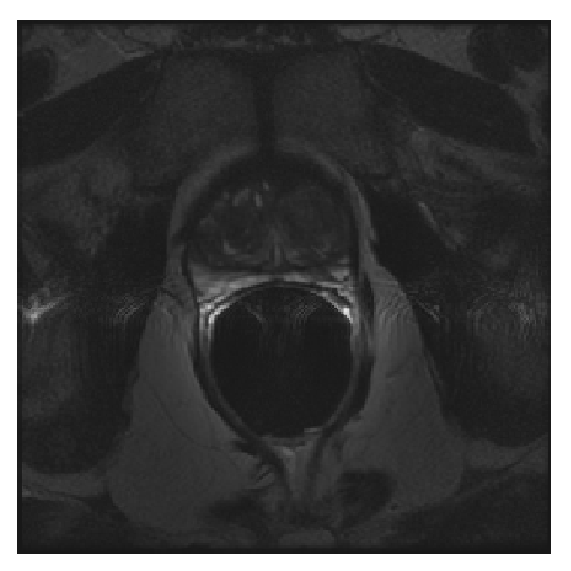
\includegraphics[width=0.3\linewidth]{3_review/figures/processing/pre-processing/bias/t2w_bias_antenna.eps}
  \caption[Non-homogeneity artifacts due to perturbation of the endorectal
  coil.]{Example of artifacts with high \acs*{si} due to perturbation from the
    endorectal coil which create non-homogeneity.}
  \label{fig:bias}
\end{figure}

% Artifacts filtering
\item[] \textbf{Bias correction}
Besides being corrupted by noise, \ac{mri} images are also affected by the
inhomogeneity of the \ac{mri} field commonly referred to as bias
field~\cite{Styner2000}.
This bias field results in a smooth variation of the \ac{si} through the image.
When an endorectal coil is used, a resulting artifact of an hyper-intense
signal is observed around the coil as depicted in \acs{fig}\,\ref{fig:bias}.
As a consequence, the \ac{si} of identical tissues varies depending on their
spatial location in the image making further processes such as segmentation,
registration, or classification more challenging~\cite{Jungke1987,Vovk2007}.
A comprehensive review of bias correction methods is proposed
in~\cite{Vovk2007}.

The model of image formation is usually formalized as:

\begin{equation}
  s(\mathbf{x}) = o(\mathbf{x})b(\mathbf{x}) + \eta(\mathbf{x}) \ ,
  \label{eq:biasmodel}
\end{equation}

\noindent where $s(\mathbf{x})$ is the corrupted \ac{si} at the pixel for the
image coordinates $\mathbf{x} = \{x,y\}$, $o(\mathbf{x})$ is the ``noise-free
signal'', $b(\mathbf{x})$ is the bias field function and $\eta(\mathbf{x})$ is
an additive white Gaussian noise.

Hence, the task of bias correction involves estimating the bias function
$b(\mathbf{x})$ in order to infer the ``signal-free bias'' $o(\mathbf{x})$.

\citeauthor{Viswanath2009} corrected this artifact on \ac{t2w}-\ac{mri}
images~\cite{Viswanath2009}, using the model proposed in~\cite{Styner2000}, in
which \citeauthor{Styner2000} model the bias field function by using a linear
combination of Legendre polynomials $f_i$ as:

\begin{align}
  \hat{b}(\mathbf{x},\mathbf{p}) & = \sum_{i=0}^{m-1} p_i f_i(\mathbf{x}) \\
  \nonumber
                                 & =  \sum_{i=0}^{l} \sum_{j=0}^{l-i} p_{ij}
                                   P_i(x) P_j(y) \ ,
                                   \label{eq:biascorr}
\end{align}

\noindent where $\hat{b}(\cdot)$ is the bias estimation with the image
coordinates $\mathbf{x} = \{x,y\}$ and the $m$ coefficients of the linear
combination $\mathbf{p} = {p_{11},\dotsc,p_{ij}}$; $m$ can be defined as
$m=(l+1)\frac{(l+2)}{2}$ where $l$ is the degree of Legendre polynomials chosen
and $P_i(\cdot)$ denotes a Legendre polynomial of degree $i$.

This family of functions offers to model the bias function as a smooth
inhomogeneous function across the image.
To estimate the set of parameters $\mathbf{p}$, a cost function is defined
which relies on the following assumptions: (i) an image is composed of $k$
regions with a mean $\mu_k$ and a variance $\sigma^{2}_{k}$ for each particular
class, and (ii) each noisy pixel belongs to one of the $k$ regions with its
\ac{si} value close to the class mean $\mu_k$.
Hence, the cost function is defined as:

\begin{equation}
  C(\mathbf{p}) = \sum_{\mathbf{x}} \prod_{k} \rho_k(s(\mathbf{x}) -
  \hat{b}(\mathbf{x},\mathbf{p}) - \mu_k) \ ,
  \label{eq:costbias}
\end{equation}

\begin{equation}
  \rho_k(x) = \frac{x^2}{x^2 + 3 \sigma_k^2} \ ,
  \label{eq:mestbias}
\end{equation}

\noindent where $\rho_k(\cdot)$ is a M-estimator allowing estimations to be
less sensitive to outliers than the usual squared distance~\cite{Li1996}.

Finally, the parameters $\mathbf{p}$ are estimated by finding the minimum of
the cost function $C(\mathbf{p})$, which was optimized using the non-linear
$(1+1)$ \ac{es} optimizer~\cite{Styner1997}.

In a later publication, \citeauthor{Viswanath2012}~\cite{Viswanath2012} as well
as \citeauthor{giannini2015fully}~\cite{giannini2015fully} corrected
\ac{t2w}-\ac{mri} using the well known N3 algorithm~\cite{Sled1998} in which
\citeauthor{Sled1998} infer the bias function using the \acp{pdf} of the signal
and bias.
Taking advantage of the logarithm property, the model in
\acs{eq}\,\eqref{eq:biasmodel} becomes additive as expressed in
\acs{eq}\,\eqref{eq:logbias}.

\begin{eqnarray}
  \log s(\mathbf{x}) & = & \log b(\mathbf{x}) + \log \left( o(\mathbf{x}) +
                           \frac{\eta(\mathbf{x})}{b(\mathbf{x})} \right) \ ,
                           \nonumber \\
                     & \approx & \log b(\mathbf{x}) + \log \hat{o}(\mathbf{x})
                                 \ , \label{eq:logbias}
\end{eqnarray}

\noindent where $\hat{o}(\mathbf{x})$ is the signal only degraded by
noise. \citeauthor{Sled1998} show that \acs{eq}\,\eqref{eq:logbias} is related
to \acp{pdf} such that:

\begin{equation}
  S(s) = B(s) * O(s) \ ,
  \label{eq:distrbias}
\end{equation}

\noindent where $S(\cdot)$, $B(\cdot)$, and $O(\cdot)$ are the \acp{pdf} of
$s(\cdot)$, $b(\cdot)$, and $o(\cdot)$, respectively.

The corrupted signal $s$ is restored by finding the multiplicative field $b$
which maximizes the frequency content of the distribution $O$.
\citeauthor{Sled1998}~\cite{Sled1998} argued that a brute-force search through
all possible fields $b$ and selecting the one which maximizes the high
frequency content of $O$ is possible but far too complex.
By assimilating the bias field distribution to be a near Gaussian distribution
as \textit{a priori}, it is then possible to infer the distribution $O$ using
the Wiener deconvolution given $B$ and $S$ and later estimate the corresponding
smooth field $b$.

\citeauthor{Lv2009} corrected the non-homogeneity in \ac{t2w}-\ac{mri}
images~\cite{Lv2009} by using the method proposed in~\cite{Madabhushi2006}.
\citeauthor{Madabhushi2006}~\cite{Madabhushi2006} proposed to correct the
\ac{mri} images by detecting the image foreground via \ac{gscale} in an
iterative manner and estimating a bias field function based on a
2\textsuperscript{nd} order polynomial model.
First, the background of the \ac{mri} image is eliminated by thresholding, in
which the threshold value is commonly equal to the mean \ac{si} of the
considered image.
Then, a seeded region growing algorithm is applied in the image foreground,
considering every thresholded pixel as a potential seed.
However, pixels already assigned to a region are not considered any more as a
potential seed.
As in seeded region growing algorithm~\cite{Shapiro2001}, two criteria are
taken into account to expand a region.
First, the region grows using a connected-neighbourhood, initially defined by
the user.
Then, the homogeneity of \ac{si} is based on a fuzzy membership function taking
into account the absolute difference of two pixel \ac{si}.
Depending on the membership value --- corresponding to a threshold which needs
to be defined --- the pixel considered is merged or not to the region.
Once this segmentation is performed, the largest region $R$ is used as a mask
to select pixels of the original image and the mean \ac{si}, $\mu_{R}$, is
computed.
The background variation $b(\mathbf{x})$ is estimated as:

\begin{equation}
  b(\mathbf{x}) = \frac{s(\mathbf{x})}{\mu_{R}}, \ \forall \mathbf{x} \in R \ ,
  \label{eq:backest}
\end{equation}

\noindent where $s(\mathbf{x})$ is the original \ac{mri} image.

Finally, a 2\textsuperscript{nd} order polynomial
$\hat{b}_{\Theta}(\mathbf{x})$ is fitted in a least-squares sense as in
\acs{eq}\,\eqref{eq:lsolv},

\begin{equation}
  \hat{\Theta} = \argmin_{\Theta} | b(\mathbf{x}) -
  \hat{b}_{\Theta}(\mathbf{x}) |^{2}, \ \forall \mathbf{x} \in R \ .
  \label{eq:lsolv}
\end{equation}

Finally, the whole original \ac{mri} image is corrected by dividing it by the
estimated bias field function $\hat{b}_{\Theta}(\mathbf{x})$.
The convergence is reached when the number of pixels in the largest region $R$
does not change significantly between two iterations.

\item[] \textbf{\Ac{si} normalization/standardization}
As discussed in the later section, segmentation or classification tasks are
usually composed of a learning stage using a set of training patients.
Hence, one can emphasize the desire to perform automatic diagnosis with a high
repeatability or in other words, one would ensure to obtain consistent \ac{si}
of tissues across patients of the same group --- i.e., healthy patients
\textit{vs.} patients with \ac{cap} --- for each \ac{mri} modality.
However, it is a known fact that variability between patients occurs during the
\ac{mri} examinations even using the same scanner, protocol or sequence
parameters~\cite{Nyul1999}.
Hence, the aim of normalization or standardization of the \ac{mri} data is to
remove the variability between patients and enforce the repeatability of the
\ac{mri} examinations.
These standardization methods are categorized either as statistical-based
standardization or organ \ac{si}-based standardization.

\citeauthor{Artan2010}~\cite{Artan2009,Artan2010},
\citeauthor{Ozer2010}~\cite{Ozer2009,Ozer2010}, and
\citeauthor{rampun2016quantitative}~\cite{,rampun2015classifying,rampun2015computer,rampun2016computer,rampun2016computerb,rampun2016quantitative}
standardized \ac{t2w}-\ac{mri}, \ac{dce}-\ac{mri}, and \ac{dw}-\ac{mri} images
by computing the \textit{standard score} (also called \textit{z-score}) of the
pixels of the \ac{pz} as:

\begin{equation}
  I_s(\mathbf{x}) = \frac{ I_r(\mathbf{x}) - \mu_{pz}}{\sigma_{pz}}, \ \forall
  \mathbf{x} \in \text{PZ} \ ,
  \label{eq:meansta}
\end{equation}

\noindent where $I_s(\mathbf{x})$ is the standardized \ac{si} with the image
coordinates $\mathbf{x} = \{x,y\}$, $I_r(\mathbf{x})$ is the raw \ac{si},
$\mu_{pz}$ is the mean \ac{si} of the \ac{pz} and $\sigma_{pz}$ is the \ac{si}
standard deviation in the \ac{pz}.
This transformation enforces the image \ac{pdf} to have a zero mean and a unit
standard deviation.
In a similar way, \citeauthor{Liu2013} normalized \ac{t2w}-\ac{mri} by making
use of the median and inter-quartile range for all the pixels~\cite{Liu2013}.

\citeauthor{lemaitre2016normalization} proposes to use the a priori that the
underlying data distribution follows a Rician distribution instead of a
Gaussian distribution~\cite{lemaitre2016normalization}.
The data are standardized by removing the mean and scaled it by dividing by the
standard-deviation which are empirically computed as follows:

\begin{equation}
  \mu_{r} = \sigma  \sqrt{\frac{\pi}{2}}\,\,L_{1/2}(-\frac{\nu^2}{2\sigma^2})  \ ,
  \label{eq:meanr}
\end{equation}

\begin{equation}
  \sigma_{r} = 2\sigma^2+\nu^2-\frac{\pi\sigma^2}{2}L_{1/2}^2\left(\frac{-\nu^2}{2\sigma^2}\right)  \ ,
  \label{eq:var}
\end{equation}

\noindent where $\nu$ and $\sigma$ are the distance between the reference point
and the center of the bivariate distribution and the scale, respectively;
$L_{1/2}$ denotes a Laguerre polynomial.

\citeauthor{Lv2009} scaled the \ac{si} of \ac{t2w}-\ac{mri} images using the
method proposed in~\cite{Nyul2000} based on \ac{pdf} matching~\cite{Lv2009}.
This approach is based on the assumption that \ac{mri} images from the same
sequence should share the same \ac{pdf} appearance.
Hence, one can approach this issue by transforming and matching the \acp{pdf}
using some statistical landmarks such as quantiles.
Using a training set, these statistical landmarks --- such as minimum,
25\textsuperscript{th} percentile, median, 75\textsuperscript{th} percentile,
and maximum --- are extracted for $N$ training images:

\begin{eqnarray}
  \Phi_{0} & = & \{ \phi_{0}^{1}, \phi_{0}^{2}, \cdots, \phi_{0}^{N} \} \ , \nonumber \\
  \Phi_{25} & = & \{ \phi_{25}^{1}, \phi_{25}^{2}, \cdots, \phi_{25}^{N} \} \ , \nonumber \\
  \Phi_{50} & = & \{ \phi_{50}^{1}, \phi_{50}^{2}, \cdots, \phi_{50}^{N} \} \ ,  \label{eq:quantileStd} \\
  \Phi_{75} & = & \{ \phi_{75}^{1}, \phi_{75}^{2}, \cdots, \phi_{75}^{N} \} \ , \nonumber \\
  \Phi_{100} & = & \{ \phi_{100}^{1}, \phi_{100}^{2}, \cdots, \phi_{100}^{N} \} \ , \nonumber
\end{eqnarray}

\noindent where $\phi_{n^\text{th}}^{i^{\text{th}}}$ is the $n^{\text{th}}$
percentile of the $i^{\text{th}}$ training image.

\citeauthor{lemaitre2016normalization} extended the use of non-parametric
transformation using an elastic transformation instead of a piecewise-linear
transformation~\cite{lemaitre2016normalization}.
They proposed to use a generic method to register functional data based on the
\ac{srsf} representation~\cite{Srivastava2011} which transforms the
Fisher-Rao metric into the conventional $\mathbb{L}^2$ metric, and thus allows
to define a cost function corresponding to an Euclidean distance between two
functions in this new representation.

\begin{figure}
  \centering
  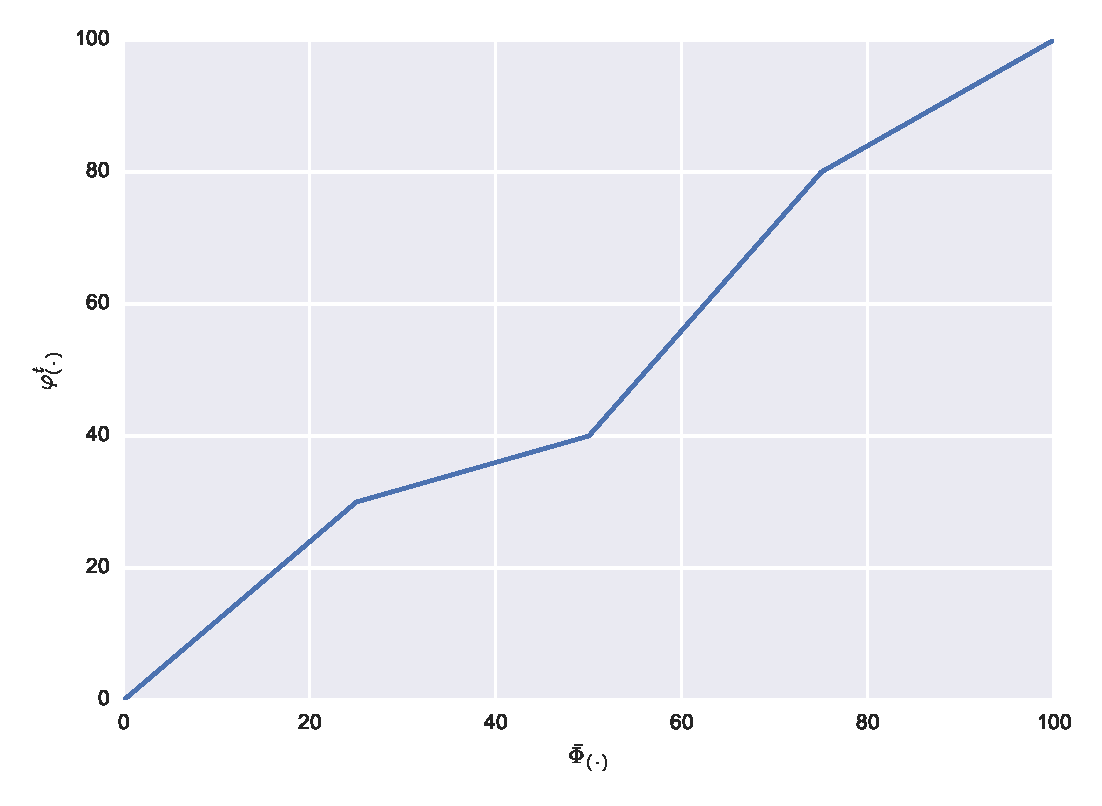
\includegraphics[width=0.7\linewidth]{3_review/figures/processing/pre-processing/normalization/linear_transform_parts.eps}
  \caption{Example of piecewise linear normalization as proposed
    in~\cite{Nyul2000}.}
  \label{fig:imnorm}
\end{figure}

Then, the mean of each statistical landmarks $\{ \bar{\Phi}_{0},
\bar{\Phi}_{25}, \bar{\Phi}_{50}, \bar{\Phi}_{75}, \bar{\Phi}_{100} \}$ is also
calculated.
Once this training stage is performed, a piecewise linear transformation
$\mathcal{T}(\cdot)$ is computed as in \acs{eq}\,\eqref{eq:linearMap}.
For each test image $t$, this transformation maps each statistical landmark
$\varphi_{(\cdot)}̂^{t}$ of the image $t$ to the pre-learned statistical
landmarks $\bar{\Phi}_{(\cdot)}$.
An example of such piecewise linear function is depicted in
\acs{fig}\,\ref{fig:imnorm}.

\begin{equation}
  \small
  \mathcal{T}(s(\mathbf{x})) =
  \begin{cases}
    \lceil \bar{\Phi}_{0}+( s(\mathbf{x}) - \varphi_{0}^{t} ) \left(
      \frac{\bar{\Phi}_{25} - \bar{\Phi}_{0}}{\varphi_{25}^{t} -
        \varphi_{0}^{t}} \right) \rceil \ , & \text{if $\varphi_{0}^{t} \leq
      s(\mathbf{x})<\varphi_{25}^{t})$} \ , \\
    \lceil \bar{\Phi}_{25}+( s(\mathbf{x}) - \varphi_{25}^{t} ) \left(
      \frac{\bar{\Phi}_{50} - \bar{\Phi}_{25}}{\varphi_{50}^{t} -
        \varphi_{25}^{t}} \right) \rceil \ , & \text{if $\varphi_{25}^{t} \leq
      s(\mathbf{x})<\varphi_{50}^{t})$} \ , \\
    \lceil \bar{\Phi}_{50}+( s(\mathbf{x}) - \varphi_{50}^{t} ) \left(
      \frac{\bar{\Phi}_{75} - \bar{\Phi}_{50}}{\varphi_{75}^{t} -
        \varphi_{50}^{t}} \right) \rceil \ , & \text{if $\varphi_{50}^{t} \leq
      s(\mathbf{x})<\varphi_{75}^{t})$} \ , \\
    \lceil \bar{\Phi}_{75}+( s(\mathbf{x}) - \varphi_{75}^{t} ) \left(
      \frac{\bar{\Phi}_{100} - \bar{\Phi}_{75}}{\varphi_{100}^{t} -
        \varphi_{75}^{t}} \right) \rceil \ , & \text{if $\varphi_{75}^{t} \leq
      s(\mathbf{x})\leq \varphi_{100}^{t})$} \ ,
  \end{cases}
  \label{eq:linearMap}
\end{equation}

\citeauthor{Viswanath2012} used a variant of the piecewise linear normalization
presented in~\cite{Madabhushi2006a}, to standardize \ac{t2w}-\ac{mri}
images~\cite{Viswanath2009,Viswanath2011,Viswanath2012}.
Instead of computing the \ac{pdf} of an entire image, a pre-segmentation of the
foreground is carried out via \ac{gscale} which has been discussed in the bias
correction section.
Once the foreground is detected, the largest region is extracted, and the
regular piecewise linear normalization is applied.

\begin{figure}
  \centering
  \hspace*{\fill}
  \subfloat[Illustration and location of the bladder on a \ac{t2w}-\ac{mri}
  image acquired with a \SI{3}{\tesla} \ac{mri} scanner]{\label{subfig:bladder}
    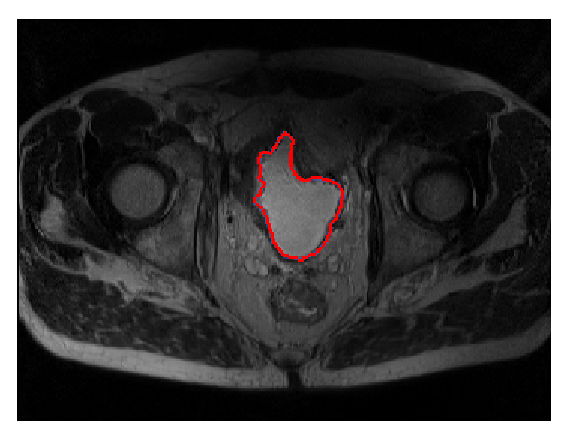
\includegraphics[width=0.3\linewidth]{3_review/figures/processing/pre-processing/niaf/t2w_bladder.eps}}
  \hfill
  \subfloat[Illustration and location of the femoral arteries on a
  \ac{t1w}-\ac{mri} image acquired with a \SI{3}{\tesla} \ac{mri}
  scanner]{\label{subfig:arteries}
    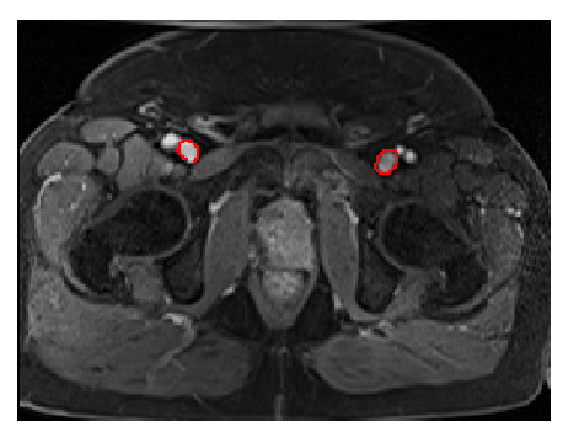
\includegraphics[width=0.3\linewidth]{3_review/figures/processing/pre-processing/niaf/t1w_arteries.eps}}
  \hspace*{\fill}
  \caption{Illustration of the two organs used in~\cite{Niaf2011,Niaf2012} to
    normalize \acs*{t2w}-\acs*{mri} and \acs*{t1w}-\acs*{mri} images.}
  \label{fig:niaf}
\end{figure}

The standardization problem can be tackled by normalizing the MRI images using
the \ac{si} of some known organs present in these images.
\citeauthor{Niaf2012} and \citeauthor{lehaire2014computer} normalized
\ac{t2w}-\ac{mri} images by dividing the original \ac{si} of the images by the
mean \ac{si} of the bladder~\cite{Niaf2011,Niaf2012,lehaire2014computer}, which
is depicted in \acs{fig}\,\ref{subfig:bladder}.
\citeauthor{giannini2015fully} also normalized the same modality but using the
signal intensity of the obturator muscle~\cite{giannini2015fully}.
Likewise, \citeauthor{Niaf2011} standardized the \ac{t1w}-\ac{mri} images using
the \ac{aif}~\cite{Niaf2011}.
They computed the \ac{aif} by taking the mean of the \ac{si} in the most
enhanced part of the common femoral arteries --- refer to
\acs{fig}\,\ref{subfig:arteries} --- as proposed in~\cite{Wiart2007}.
Along the same line, \citeauthor{samarasinghe2016semi} normalized the \ac{si}
of lesion regions in \ac{t1w}-\ac{mri} using the mean intensity of the prostate
gland in the same modality~\cite{samarasinghe2016semi}.

\end{enumerate}

\subsubsection{\acs*{mrsi} modalities}\label{subsubsec:ch3:mriprepro}

As presented in \acs{sec}\,\ref{subsec:chp2:imaging:mrsi}, \ac{mrsi} is a
modality related to a one dimensional signal.
Hence, specific pre-processing steps for this type of signals have been applied
instead of standard signal processing methods.

\setenumerate{listparindent=\parindent,itemsep=10px}
\setlist{noitemsep}
\begin{enumerate}[leftmargin=*]

\begin{figure}
  \centering
  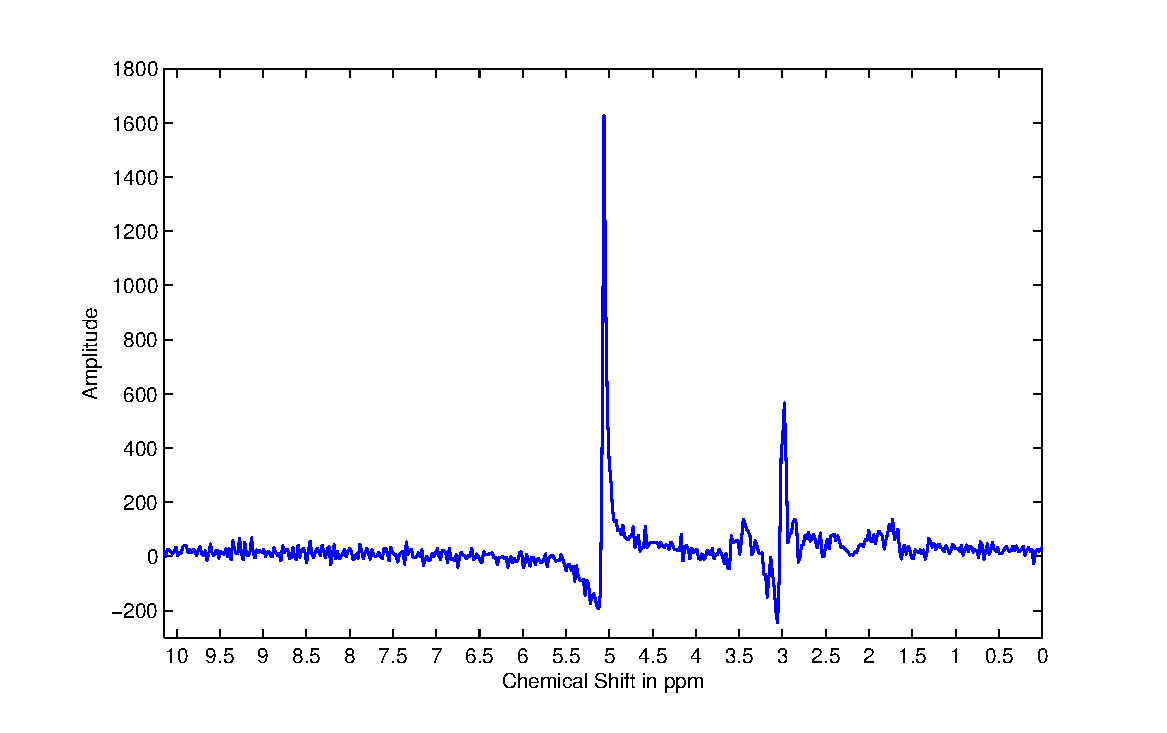
\includegraphics[width=0.7\linewidth]{3_review/figures/processing/pre-processing/phase/phase.eps}
  \caption[Illustration of phase malignant in an \acs*{mrsi}
  spectra.]{Illustration of phase misalignment in an \acs*{mrsi} spectra
    acquired with a \SI{3}{\tesla} \acs*{mrsi} scanner. Note the distortion of
    the signal specially visible for the water and citrate peaks visible at
    \SI{5}{\ppm} and \SI{3}{\ppm}, respectively}
  \label{fig:phase}
\end{figure}

\item[] \textbf{Phase correction}
Acquired \ac{mrsi} spectra suffer from zero-order and first-order phase
misalignment~\cite{Chen2002,Osorio-Garcia2012} as depicted in
\acs{fig}\,\ref{fig:phase}.
\citeauthor{Parfait2012} and \citeauthor{trigui2017automatic} used a method
proposed by \citeauthor{Chen2002} where the phase of \ac{mrsi} signal is
corrected based on entropy minimization in the frequency
domain~\cite{Parfait2012,trigui2016classification,trigui2017automatic}.
The corrected \ac{mrsi} signal $o(\xi)$ can be expressed as:

\begin{eqnarray}
  \Re(o(\xi)) & = & \Re(s(\xi))\cos(\Phi(\xi)) - \Im(\xi)\sin(\Phi(\xi)) \ ,
                    \nonumber  \\
  \Im(o(\xi)) & = & \Im(s(\xi))\cos(\Phi(\xi)) + \Re(\xi)\sin(\Phi(\xi)) \ ,
                    \nonumber \\
  \Phi(\xi) & = & \phi_0 + \phi_1 \frac{\xi}{N} \ , \label{eq:mrsiphcorr}
\end{eqnarray}

\noindent where $\Re(\cdot)$ and $\Im(\cdot)$ are the real and imaginary part
of the complex signal, respectively, $s(\xi)$ is the corrupted \ac{mrsi}
signal, $\phi_0$ and $\phi_1$ are the zero-order and first-order phase
correction terms respectively and $N$ is the total number of samples of the
\ac{mrsi} signal.

\citeauthor{Chen2002} tackled this problem as an optimization in which $\phi_0$
and $\phi_1$ have to be inferred.
Hence, the simplex Nelder-Mead optimizer~\cite{Nelder1965} is used to minimize
the following cost function based on the \textit{Shannon entropy} formulation:

\begin{equation}
  \hat{\Phi} = \argmin_{\Phi} \left[ - \sum \Re(s'(\xi)) \ln \Re(s'(\xi)) +
    \lambda \|\Re(s(\xi))\|_2 \right] \ ,
  \label{eq:phcost}
\end{equation}

\noindent where $s'(\xi)$ is the first derivative of the corrupted signal
$s(\xi)$ and $\lambda$ is a regularization parameter.
Once the best parameter $\Phi$ vector is obtained, the \ac{mrsi} signal is
corrected using \acs{eq}\,\eqref{eq:mrsiphcorr}.

\begin{figure}
  \centering
  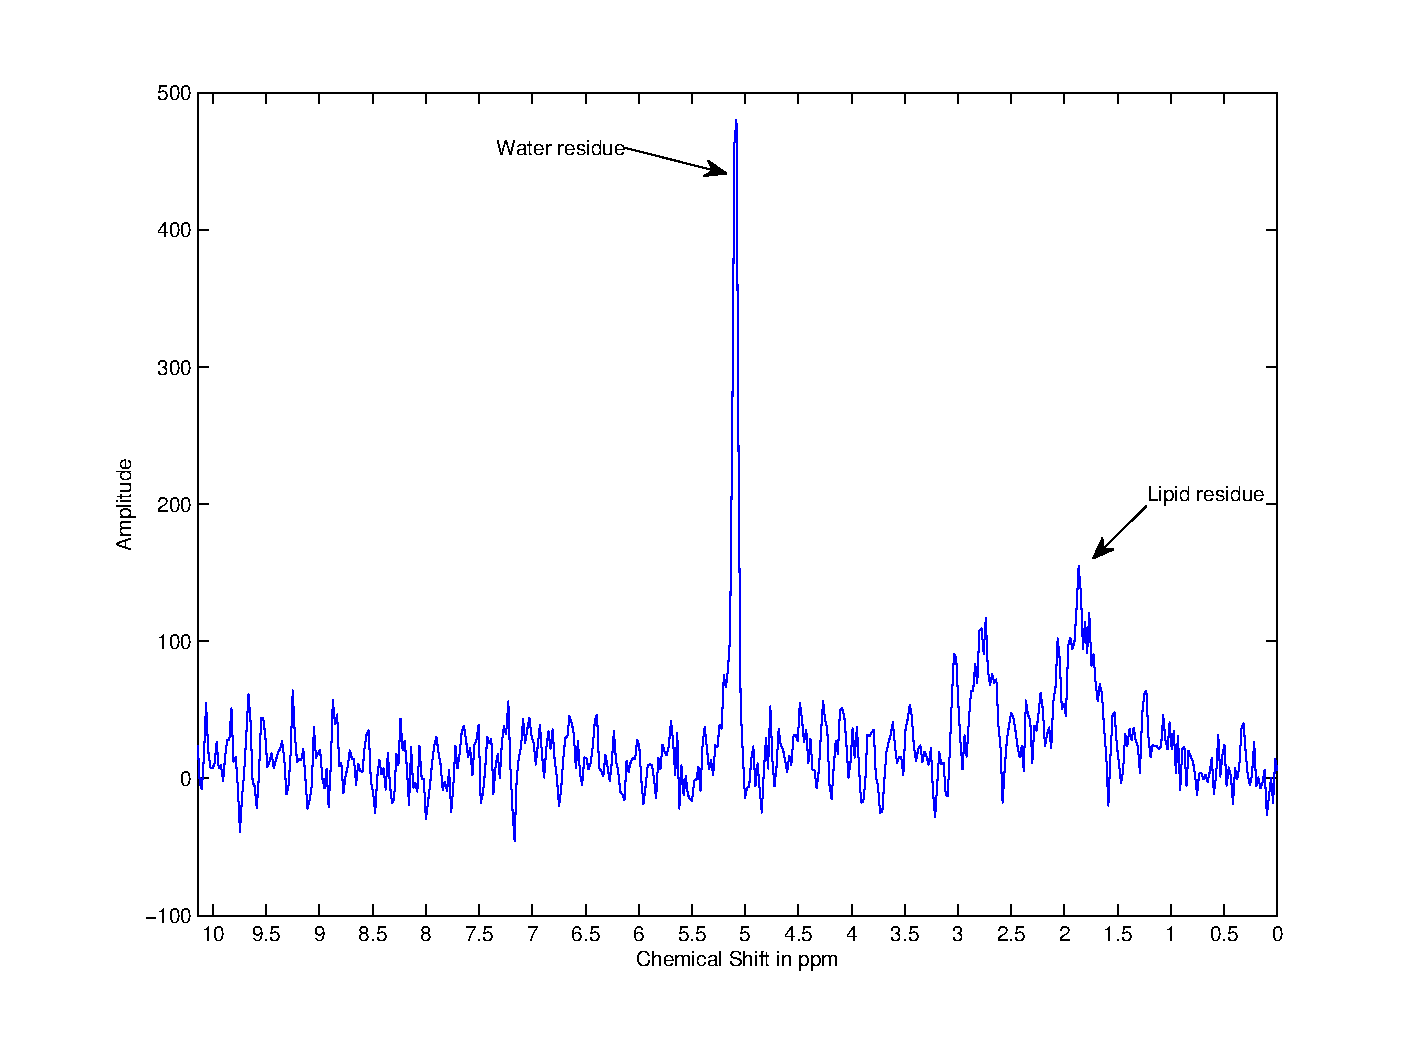
\includegraphics[width=0.7\linewidth]{3_review/figures/processing/pre-processing/water/water_fat.eps}
  \caption[Illustration of water and fat residues in \acs*{mrsi} signal after
  suppression during acquisition.]{Illustration of the residues of water and
    fat even after their suppression during the acquisition protocol. The
    acquisition has been carried out with a \SI{3}{\tesla} \acs*{mri}.}
  \label{fig:waterfat}
\end{figure}

\item[] \textbf{Water and lipid residuals filtering}
The water and lipid metabolites occur in much higher concentrations than the
metabolites of interest, namely choline, creatine, and
citrate~\cite{Zhu2010,Osorio-Garcia2012}.
Fortunately, specific \ac{mrsi} sequences have been developed in order to
suppress water and lipid metabolites using pre-saturation
techniques~\cite{Zhu2010}.
However, these techniques do not perfectly remove water and lipids peaks and
some residuals are still present in the \ac{mrsi} spectra as illustrated in
\ac{fig}\,\ref{fig:waterfat}.
Therefore, different post-processing methods have been proposed to enhance the
quality of the \ac{mrsi} spectra by removing these residuals.
For instance, \citeauthor{Kelm2007}~\cite{Kelm2007} used the HSVD algorithm
proposed by \citeauthor{Pijnappel1992}~\cite{Pijnappel1992} which models the
\ac{mrsi} signal by a sum of exponentially damped sine waves in the time domain
as \acs{eq}\,\eqref{eq:fidsig}.

\begin{equation}
  s(t) = \sum_{k=1}^{K} a_{k}\exp(i \phi_k) \exp( -d_{k} + i 2 \pi f_{k} ) t +
  \eta(t) \ ,
  \label{eq:fidsig}
\end{equation}

\noindent where $a_k$ is the amplitude proportional to the metabolite
concentration with a resonance frequency $f_{k}$, $d_k$ represents the damping
factor of the exponential, $\phi_k$ is the first-order phase, and $\eta(t)$ is
a complex white noise.

The ``noise-free signal'' can be found using the \ac{svd}
decomposition~\cite{Pijnappel1992}.
Therefore, the noisy signal is reorganized inside a Hankel matrix $H$.
It can be shown that the signal is considered as a ``noise-free signal'' if the
rank of $H$ is equal to rank $K$.
However, due to the presence of noise, $H$ is in fact a full rank matrix.
Thus, to recover the ``noise-free signal'', the rank of $H$ is truncated to $K$
using its \ac{svd} decomposition.
Hence, knowing the cut off frequencies of water --- i.e., \SI{4.65}{\ppm} ---
and lipid --- i.e., \SI{2.2}{\ppm} --- metabolites, their corresponding peaks
are reconstructed and subtracted from the original signal~\cite{Laudadio2002}.

\item[] \textbf{Baseline correction}
Sometimes, the problem discussed in the above section regarding the lipid
molecules is not addressed simultaneously with water residuals suppression.
Lipids and macro-molecules are known to affect the baseline of the \ac{mrsi}
spectra, causing errors while quantifying metabolites, especially the citrate
metabolite.

\citeauthor{Parfait2012} made the comparison of two different methods to detect
the baseline and correct the \ac{mrsi} spectra~\cite{Parfait2012} which are
based on~\cite{Lieber2003,Devos2004}.
\citeauthor{Lieber2003} corrected the baseline in the frequency domain by
fitting a low degree polynomial $p(x)$ --- e.g., 2\textsuperscript{nd} or
3\textsuperscript{rd} degree --- to the \ac{mrsi} signal $s(x)$ in a
least-squares sense~\cite{Lieber2003}.
Then, the values of the fitted polynomial are re-assigned as:

\begin{equation}
  p_f(x) =
  \begin{cases}
    p(x) \ , & \text{if $p(x) \leq s(x)$} \ , \\
    s(x) \ , & \text{if $p(x) > s(x)$} \ . \\
  \end{cases}
  \label{eq:lieber}
\end{equation}

Finally, this procedure of fitting and re-assignment is repeated on $p_f(x)$
until a stopping criterion is reached.
The final polynomial function is subtracted from the original signal $s(x)$ to
correct it.
\citeauthor{Parfait2012}~\cite{Parfait2012} modified this algorithm by
convolving a Gaussian kernel to smooth the \ac{mrsi} signal instead of fitting
a polynomial function, keeping the rest of the algorithm identical.
Unlike~\citeauthor{Lieber2003}~\cite{Lieber2003},
\citeauthor{Devos2004}~\cite{Devos2004} corrected the baseline in the time
domain by multiplying the \ac{mrsi} signal by a decreasing exponential function
as:

\begin{equation}
  c(t) = \exp (- \beta t) \ ,
  \label{eq:devos}
\end{equation}

\noindent with a typical $\beta$ value of $0.15$.
However, \citeauthor{Parfait2012} concluded that the method proposed
in~\cite{Lieber2003} outperformed the one in~\cite{Devos2004}.
The later study of \citeauthor{trigui2017automatic} used this conclusion and
adopted the same method~\cite{trigui2016classification,trigui2017automatic}.

The previous baseline correction methods does not provide an optimal solution
since the iterative low-pass filter enforces too much the smoothness of the
baseline.
\citeauthor{xi2008baseline} proposed a baseline detection derived from a
parametric smoothing model~\cite{xi2008baseline}.
The \ac{nmr} signal is formalized as a sum of a pure signal, the baseline
function, and an additive Gaussian noise such as:

\begin{equation}
  y_i = b_i + \mu_i e^{n_i} + \varepsilon_i \ ,
  \label{eq:methodBaselineDetectionModel}
\end{equation}

\noindent where $y_i$ is the \ac{nmr} signal, $b_i$ is the baseline, $\mu_i$ is
the true signal, and $n_i$ and $\varepsilon_i$ are Gaussian noises.

\citeauthor{xi2008baseline} propose to find the baseline function through an
iterative optimization by maximizing the following cost function:

\begin{equation}
  F(b) = \sum_{i = 1}^{N} b_i - \frac{A^{*} N^4}{\sigma} \sum_{i = 1}^{N} (b_{i+1} + b_{i-1} - 2 b_i)^2 - \frac{1.25 B^{*}}{\sigma} \sum_{i = 1}^{N} (b_i - \gamma_i)^2 g(b_i - \gamma_i) \ ,
  \label{eq:methodBaselineDetectionCostFunction}
\end{equation}

\noindent where $g(b_i - \gamma_i)$ is the Heaviside function, $A^*$ and $B^*$
are the terms controlling the smoothness and negative penalties, respectively,
$\sigma$ is an estimation of the standard deviation of the noise, and $N$ is
the total number of points in the \ac{mrsi} signal.

The standard deviation of the noise $\sigma$ is estimated as
in~\cite{xi2008baseline}, and the $A^{*}$ and $B^{*}$ are empirically set to $5
\times 10^{-6}$ and $100$, respectively, for all the \ac{mrsi} signal.
This method was used in the work of
\citeauthor{Lemaitre2016thesis}~\cite{Lemaitre2016thesis}.

In the contemporary work of \citeauthor{Tiwari2012}~\cite{Tiwari2012}, the
authors detected the baseline using a local non-linear fitting method avoiding
regions with significant peaks, which have been detected using an
experimentally parametric signal-to-noise ratio set to a value larger than
\SI{5}{\decibel}.

\begin{figure}
  \centering
  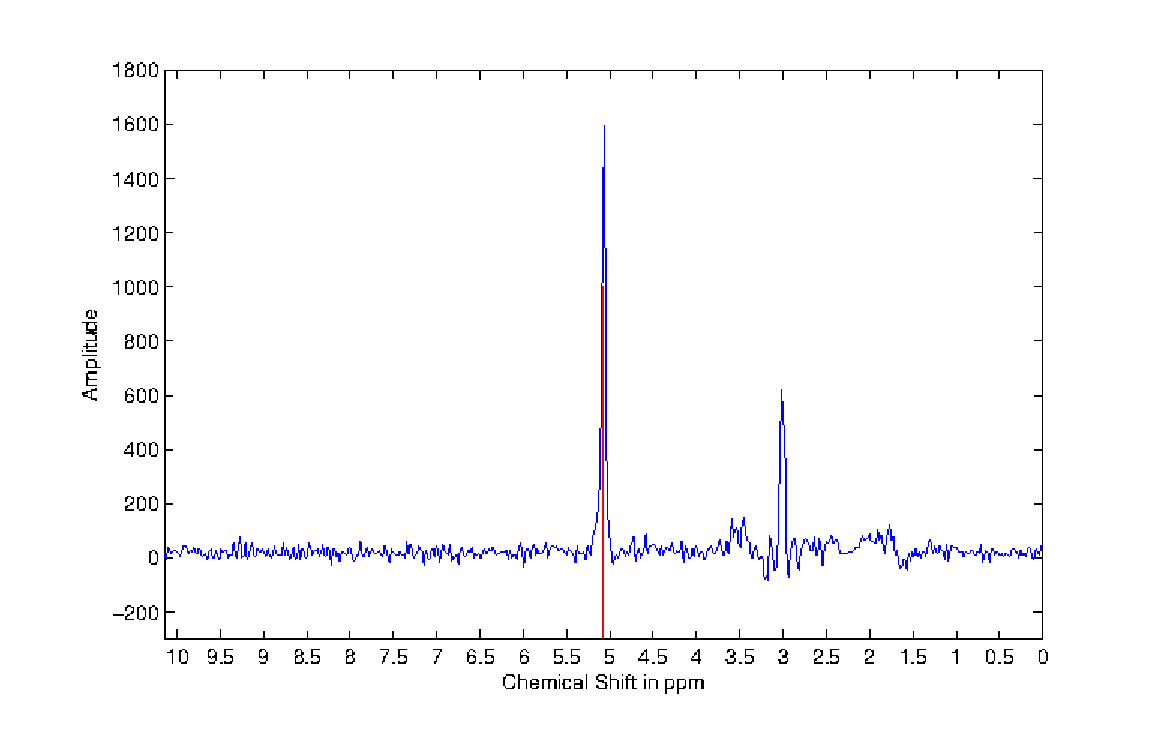
\includegraphics[width=0.7\linewidth]{3_review/figures/processing/pre-processing/frequency/frequency.eps}
  \caption[Illustration of frequency misalignment in a \acs*{mrsi}
  spectra.]{Illustration of frequency misalignment in a \acs*{mrsi} spectra
    acquired with a \SI{3}{\tesla} \acs*{mrsi} scanner. The water peak is known
    to be aligned at \SI{4.65}{\ppm}. However, it can be seen that the peak on
    this spectra is aligned at around \SI{5.1}{\ppm}.}
  \label{fig:frequency}
\end{figure}

\item[] \textbf{Frequency alignment}
Due to variations of the experimental conditions, a frequency shift is commonly
observed in the \ac{mrsi} spectra~\cite{Chen2002,Osorio-Garcia2012} as depicted
in \acs{fig}\,\ref{fig:frequency}.
\citeauthor{Tiwari2012}~\cite{Tiwari2012} corrected this frequency shift by
first detecting known metabolite peaks such as choline, creatine, or citrate
and minimizing the frequency error between the experimental and theoretical
values for each of these peaks~\cite{Tiwari2012}.

\item[] \textbf{Normalization}
The \ac{nmr} spectra is subject to variations due to intra-patient variations
and non homogeneity of the magnetic field.
\citeauthor{Parfait2012} as in~\cite{Devos2004} compared two methods to
normalize \ac{mrsi} signal~\cite{Parfait2012}.
In each method, the original \ac{mrsi} spectra is divided by a normalization
factor, similar to the intensity normalization described earlier.
The first approach consists in estimating the water concentration from an
additional \ac{mrsi} sequence where the water has not been suppressed.
The estimation is performed using the previously HSVD algorithm.
The second approach does not require any additional acquisition and is based on
the L$_2$ norm of the \ac{mrsi} spectra $\|s(\xi)\|_2$.
It should be noted that both \citeauthor{Parfait2012} and
\citeauthor{Devos2004} concluded that the L$_2$ normalization is the most
efficient method~\cite{Parfait2012}.
Lately, \citeauthor{trigui2017automatic} used the L$_2$ normalization in their
framework~\cite{trigui2016classification,trigui2017automatic}.

\end{enumerate}

\subsubsection{Summary}

The different pre-processing methods are summarized in \acs{tab}~\ref{tab:summary-preproc}.

\begin{table}
  \caption{Overview of the pre-processing methods used in \acs*{cad} systems.}
  \centering
  \begin{tabular}{l r}
    \toprule
    \textbf{Pre-processing operations} & \textbf{References} \\
    \midrule
    \textbf{\ac{mri} pre-processing:} & \\
    \quad Noise filtering: &  \\
    \quad \quad $\bullet$ Anisotropic median-diffusion filtering &
                                                                   \cite{rampun2015classifying,rampun2015computer,rampun2016computer,rampun2016computerb,rampun2016quantitative}
    \\
    \quad \quad $\bullet$ Gaussian filtering & \cite{samarasinghe2016semi}  \\
    \quad \quad $\bullet$ Median filtering & \cite{Ozer2009,Ozer2010}  \\
    \quad \quad $\bullet$ Wavelet-based filtering &
                                                    \cite{Ampeliotis2007,Ampeliotis2008,Lopes2011}
    \\ \\ [-1.5ex]
    \quad Bias correction: & \\
    \quad \quad $\bullet$ Parametric methods &
                                               \cite{Lv2009,Viswanath2009,giannini2015fully}
    \\
    \quad \quad $\bullet$ Non-parametric methods & \cite{Viswanath2011} \\ \\
    [-1.5ex]
    \quad Standardization: & \\
    \quad \quad $\bullet$ Statistical-based normalization: &
                                                             \cite{Artan2009,Artan2010,Lv2009,Ozer2009,Ozer2010,rampun2015classifying,rampun2015computer,rampun2016computer,rampun2016computerb,rampun2016quantitative,Viswanath2009,Viswanath2011,Viswanath2012,Lemaitre2016thesis}
    \\
    \quad \quad $\bullet$ Organ \ac{si}-based normalization &
                                                              \cite{Niaf2011,Niaf2012,lehaire2014computer,samarasinghe2016semi}
    \\ \\ [-1.5ex]
    \textbf{\ac{mrsi} pre-processing:} & \\ \\ [-1.5ex]
    \quad Phase correction &
                             \cite{Parfait2012,trigui2016classification,trigui2017automatic,Lemaitre2016thesis}
    \\
    \quad Water and lipid residuals filtering & \cite{Kelm2007} \\
    \quad Baseline correction &
                                \cite{Parfait2012,Tiwari2012,trigui2016classification,trigui2017automatic,Lemaitre2016thesis}
    \\
    \quad Frequency alignment &
                                \cite{Tiwari2012,trigui2016classification,trigui2017automatic,Lemaitre2016thesis}
    \\
    \quad Normalization & \cite{Parfait2012,trigui2016classification,trigui2017automatic,Lemaitre2016thesis} \\
    \bottomrule
  \end{tabular}
  \label{tab:summary-preproc}
\end{table}
